% Revised Results section. Generated by make_paper_text.py from results/*.json -- do not edit numbers by hand.
% Tables and figures are in paper_out/tables and paper_out/figures (make_outputs.py).
% Tables hardware and retrieval are input here; move them to the Setup section if preferred.
\section{Results}
\label{sec:results}

All numbers in this section come from one cached run of every path on every query
(8,150 validation questions from DocVQA and InfographicVQA over 1,786 page images) on a single
GeForce RTX 4090 (Table~\ref{tab:hardware}). Costs are measured, not priced: GPU-seconds, energy from NVML, and wall-clock
latency per query. Routers are trained and evaluated on 5 page-grouped 60/20/20 splits, so no page
appears in more than one split; each test split holds 1,548--1,653 questions. Unless marked
otherwise, policy results are means ($\pm$ standard deviation) over the 5 seeds; figures marked
``seed 1'' show the first split.

\begin{table}[t]
\centering
\caption{Workstation used for every measurement except multi-GPU index sharding (Table~\ref{tab:hardware_multigpu}): hardware, software and model revisions.}
\label{tab:hardware}
\begin{tabular}{ll}
\toprule
\textbf{Component} & \textbf{Value} \\
\midrule
GPU & 1 $\times$ NVIDIA GeForce RTX 4090 (24\,GiB, power limit 450\,W) \\
Driver / CUDA / cuDNN & 572.61 / 12.8 / 9.19.0 \\
CPU & AMD Ryzen 9 5950X 16-Core Processor \\
CPU threads / RAM & 32 / 64\,GiB \\
OS / Python & Windows 11 (build 26200) / 3.11.17 \\
PyTorch / Transformers & 2.11.0+cu128 / 5.18.0 \\
colpali-engine / docTR & 0.3.18 / 1.1.0 \\
sentence-transformers / scikit-learn & 6.1.0 / 1.9.1 \\
rank-bm25 / qwen-vl-utils / datasets & 0.2.2 / 0.0.14 / 5.0.1 \\
\texttt{Qwen2.5-VL-7B-Instruct} revision & \texttt{cc59489} \\
\texttt{colpali-v1.3} revision & \texttt{b5c6dd6} \\
\texttt{colpaligemma-3b-pt-448-base} revision & \texttt{30ab955} \\
\texttt{all-mpnet-base-v2} revision & \texttt{e8c3b32} \\
Interconnect & single GPU (multi-GPU sharding: Table~\ref{tab:hardware_multigpu}) \\
\bottomrule
\end{tabular}
\end{table}


\subsection{Cost and answer quality of each path}
\label{sec:res-paths}

All three paths use the same generator (Qwen2.5-VL-7B-Instruct, greedy decoding). The text path reads the top-3
BM25 pages of OCR text; the visual path reads the top-1 ColPali page image (at most 1280 visual
tokens); the hybrid path reads both. Over all 8,150 questions, always-text reaches ANLS 0.367 at
0.43 GPU-s per query, always-visual 0.546 at 0.62 GPU-s, and always-hybrid
0.570 at 1.01 GPU-s (329\,J).
With a shared local generator the text path is therefore \emph{not} the cheap path the submitted version
assumed: OCR text costs about as many input tokens as a page image, and the text path is much less accurate.
The real cost differences are between one context and two (hybrid costs 1.6$\times$ the visual path and
2.3$\times$ the text path) and the size of the visual index at scale (Section~\ref{sec:res-scale}).
In 35\% of queries every path fails. For 76\% of these, no path had the gold page in its
context (page recall@1 is 0.44 for BM25 and 0.57 for ColPali; Table~\ref{tab:retrieval}). No router
can recover these queries; they bound every policy.

\begin{table}[t]
\centering
\caption{Page retrieval over each dataset's page pool. ColPali per query: encode 46\,ms + score 1.1\,ms (p50); index build 210\,s for 1786 pages, 450\,MB.}
\label{tab:retrieval}
\begin{tabular}{lrrrrr}
\toprule
\textbf{Retriever} & \textbf{R@1} & \textbf{R@3} & \textbf{R@5} & \textbf{R@10} & \textbf{MRR} \\
\midrule
BM25 (docTR text) & 0.439 & 0.546 & 0.586 & 0.633 & 0.507 \\
ColPali v1.3 & 0.573 & 0.697 & 0.749 & 0.798 & 0.651 \\
\bottomrule
\end{tabular}
\end{table}


\subsection{Outcome-based route labels}
\label{sec:res-labels}

Route labels are now derived from measured outcomes: the label of a query is the path that maximises
$\mathrm{ANLS} - \lambda \cdot \mathrm{cost}$, with ties broken towards the cheaper path (Table~\ref{tab:labels}).
The keyword labels used in the submitted version agree with these outcome labels on 68.5\% of queries,
with Cohen's $\kappa = 0.01$, i.e.\ no agreement beyond chance; the keyword rule sends 97\% of
queries to the text path. Routing accuracy against keyword labels therefore says nothing about cost or answer
quality, and we no longer report it.

\begin{table}[t]
\centering
\caption{Outcome-based route labels on the seed-1 split (utility label at $\lambda$=0.1; threshold label = cheapest path with ANLS $\geq$ 0.5). The submitted keyword labels agree with the utility labels on 68.5\% of queries (Cohen's $\kappa$ = 0.01).}
\label{tab:labels}
\begin{tabular}{lrrr}
\toprule
\textbf{Split} & \textbf{Text} & \textbf{Visual} & \textbf{Hybrid} \\
\midrule
train & 3377 & 1398 & 114 \\
val & 1199 & 410 & 46 \\
test & 1099 & 457 & 50 \\
train (threshold) & 3583 & 1235 & 71 \\
val (threshold) & 1270 & 357 & 28 \\
test (threshold) & 1176 & 401 & 29 \\
\bottomrule
\end{tabular}
\end{table}


\subsection{Routing policies}
\label{sec:res-policies}

Table~\ref{tab:main_results} compares fixed policies, the submitted keyword rule, simple learned baselines,
CAVR, the content-aware CAVR-CE and the per-query oracle. All router costs include the router's own measured
overhead and, where the router reads ColPali scores, ColPali retrieval for every query.

CAVR on question embeddings alone (ANLS 0.542 $\pm$ 0.012) shows no significant difference from always-visual:
on every seed the 95\% bootstrap interval of the ANLS difference includes zero and lies within
$\pm$0.007, while CAVR uses 4\% more GPU. The question text alone does not predict
which path will succeed.
CAVR-CE adds what is available before generation: an mpnet cross-encoder reads the question with the
best-matching OCR passages of the retrieved pages, plus retrieval scores and ColPali per-token match statistics.
With $\lambda$ chosen on each seed's validation split (the cheapest $\lambda$ within 0.005 ANLS of always-hybrid),
CAVR-CE reaches ANLS 0.557 $\pm$ 0.013 at 0.716 GPU-s per query, against
0.566 $\pm$ 0.018 at 1.009 GPU-s for always-hybrid: 29\% less GPU compute
(25--36\% across seeds; Table~\ref{tab:router_ce_tests}).
The price is a small ANLS loss: CAVR-CE is lower than always-hybrid on 4 of 5 seeds
(mean difference $-0.008$, range $-0.015$ to $+0.001$), and the 95\% bootstrap interval
excludes zero on 1 of 5 seeds. On exact match, the difference is not significant on
5 of 5 seeds (McNemar $p = 0.098$--$0.74$).
Against always-visual, CAVR-CE gains $+0.012$ to $+0.018$ ANLS (bootstrap interval above zero on
5 of 5 seeds; McNemar on exact match $p \le 0.029$ on 5 of 5 seeds)
for 15\% more GPU.

The per-query oracle reaches ANLS 0.630 $\pm$ 0.014 at only 0.486 GPU-s, so substantial headroom
remains. It is limited by prediction: CAVR-CE predicts per-path success with a mean AUC of 0.842
(0.839 for gradient boosting on the same tabular features), and a learning curve over 25--100\% of the
training pages (2 seeds) rises only from 0.826 to 0.841.

\begin{table}[t]
\centering
\caption{Routing policies on held-out test pages (mean $\pm$ std over 5 seeds, $\lambda$ = 0.1). Cost is measured per query on one RTX 4090 including router overhead. p: McNemar (EM) vs CAVR, seed 1.}
\label{tab:main_results}
\begin{tabular}{lrrrrrr}
\toprule
\textbf{Policy} & \textbf{ANLS} & \textbf{EM} & \textbf{GPU-s} & \textbf{Energy (J)} & \textbf{p95 lat. (s)} & \textbf{p} \\
\midrule
Always text & 0.364 $\pm$ 0.017 & 0.312 $\pm$ 0.015 & 0.434 $\pm$ 0.002 & 144 $\pm$ 1 & 0.74 $\pm$ 0.01 & 3.5e-46 \\
Always visual & 0.542 $\pm$ 0.012 & 0.498 $\pm$ 0.014 & 0.621 $\pm$ 0.005 & 170 $\pm$ 1 & 0.95 $\pm$ 0.01 & 1 \\
Always hybrid & 0.566 $\pm$ 0.018 & 0.517 $\pm$ 0.019 & 1.009 $\pm$ 0.003 & 328 $\pm$ 1 & 1.39 $\pm$ 0.02 & 0.00027 \\
Keyword rule (submitted) & 0.372 $\pm$ 0.018 & 0.320 $\pm$ 0.015 & 0.443 $\pm$ 0.003 & 146 $\pm$ 1 & 0.76 $\pm$ 0.02 & 1.6e-42 \\
Keyword rule (regex fixed) & 0.372 $\pm$ 0.019 & 0.321 $\pm$ 0.016 & 0.443 $\pm$ 0.003 & 146 $\pm$ 1 & 0.77 $\pm$ 0.03 & 4.1e-42 \\
Random (equal budget) & 0.536 $\pm$ 0.012 & 0.492 $\pm$ 0.012 & 0.637 $\pm$ 0.020 & 179 $\pm$ 8 & 1.06 $\pm$ 0.09 & -- \\
Logistic regression & 0.404 $\pm$ 0.020 & 0.354 $\pm$ 0.020 & 0.475 $\pm$ 0.004 & 148 $\pm$ 1 & 0.83 $\pm$ 0.02 & 2.5e-36 \\
kNN quality & 0.544 $\pm$ 0.012 & 0.498 $\pm$ 0.013 & 0.717 $\pm$ 0.007 & 208 $\pm$ 3 & 1.25 $\pm$ 0.02 & 1 \\
CAVR (class head only) & 0.375 $\pm$ 0.025 & 0.324 $\pm$ 0.022 & 0.453 $\pm$ 0.014 & 146 $\pm$ 2 & 0.77 $\pm$ 0.04 & 7.8e-34 \\
CAVR & 0.542 $\pm$ 0.012 & 0.497 $\pm$ 0.014 & 0.645 $\pm$ 0.020 & 178 $\pm$ 7 & 1.06 $\pm$ 0.10 & -- \\
CAVR + BM25 scores & 0.545 $\pm$ 0.014 & 0.500 $\pm$ 0.015 & 0.651 $\pm$ 0.021 & 181 $\pm$ 9 & 1.07 $\pm$ 0.09 & 0.12 \\
CAVR + BM25 + ColPali scores & 0.549 $\pm$ 0.010 & 0.503 $\pm$ 0.010 & 0.679 $\pm$ 0.022 & 194 $\pm$ 9 & 1.19 $\pm$ 0.03 & 1 \\
CAVR-CE (content-aware) & 0.557 $\pm$ 0.013 & 0.512 $\pm$ 0.013 & 0.694 $\pm$ 0.019 & 196 $\pm$ 7 & 1.22 $\pm$ 0.04 & 0.018 \\
CAVR-CE, val-chosen $\lambda$ & 0.557 $\pm$ 0.013 & 0.512 $\pm$ 0.013 & 0.716 $\pm$ 0.038 & 205 $\pm$ 15 & 1.24 $\pm$ 0.06 & 0.0049 \\
Per-query oracle & 0.630 $\pm$ 0.014 & 0.581 $\pm$ 0.016 & 0.486 $\pm$ 0.004 & 150 $\pm$ 1 & 0.87 $\pm$ 0.01 & 4.6e-41 \\
\bottomrule
\end{tabular}
\end{table}

\begin{table}[t]
\centering
\caption{CAVR-CE with $\lambda$ chosen on each seed's validation split (cheapest $\lambda$ within 0.005 ANLS of always-hybrid on val), against always-hybrid and always-visual on test. GPU-s include ColPali for every query and the router's measured overhead.}
\label{tab:router_ce_tests}
\begin{tabular}{lrrrrrrrrrr}
\toprule
\textbf{Seed} & \textbf{$\lambda$} & \textbf{ANLS} & \textbf{Hybrid ANLS} & \textbf{GPU-s} & \textbf{Hybrid GPU-s} & \textbf{Saving} & \textbf{$\Delta$ANLS vs hybrid [95\% CI]} & \textbf{McNemar p} & \textbf{$\Delta$ANLS vs visual} & \textbf{McNemar p} \\
\midrule
1 & 0.075 & 0.566 & 0.578 & 0.731 & 1.007 & 27\% & $-0.012$ [$-0.023$, $+0.001$] & 0.12 & $+0.017$ & 0.004 \\
2 & 0.1 & 0.577 & 0.592 & 0.705 & 1.012 & 30\% & $-0.015$ [$-0.027$, $-0.004$] & 0.11 & $+0.015$ & 0.029 \\
3 & 0.01 & 0.538 & 0.540 & 0.739 & 1.006 & 27\% & $-0.002$ [$-0.013$, $+0.009$] & 0.56 & $+0.012$ & 0.0018 \\
4 & 0.03 & 0.552 & 0.552 & 0.757 & 1.007 & 25\% & $+0.001$ [$-0.010$, $+0.012$] & 0.74 & $+0.016$ & 0.029 \\
5 & 0.2 & 0.554 & 0.567 & 0.646 & 1.012 & 36\% & $-0.013$ [$-0.025$, $-0.002$] & 0.098 & $+0.018$ & 0.0046 \\
\bottomrule
\end{tabular}
\end{table}


\subsection{Runtime budget control}
\label{sec:res-lambda}

The decision rule $\arg\max_p \hat{q}_p - \lambda c_p$ takes the cost weight $\lambda$ at serving time, so one
trained router covers a range of budgets without retraining. Sweeping $\lambda$ from 1 to 0 moves CAVR-CE from
ANLS 0.502 at 0.56 GPU-s to 0.564 at 0.84 GPU-s (mean over seeds;
Figure~\ref{fig:pareto} shows seed 1). Table~\ref{tab:load_test_ops} gives the serving capacity of each operating
point on seed 1.

\begin{figure}[t]
  \centering
  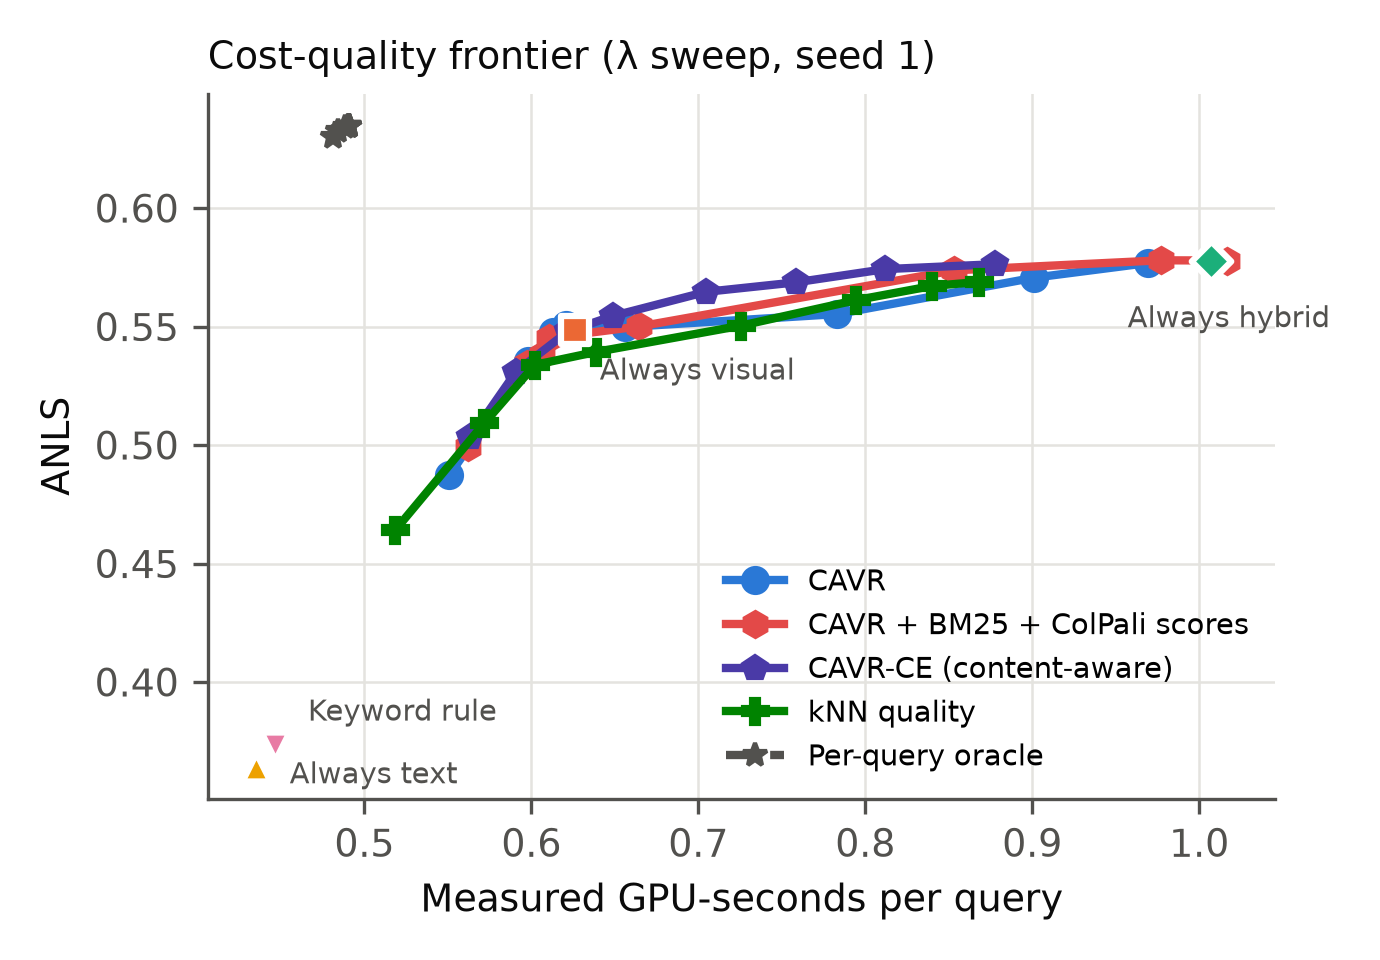
\includegraphics[width=\columnwidth]{figures/pareto.png}
  \caption{Cost--quality frontier of each router as $\lambda$ is swept (seed 1), with fixed policies and the
  per-query oracle. Costs are measured GPU-seconds per query including router overhead.}
  \label{fig:pareto}
\end{figure}

\subsection{Confidence-based escalation}
\label{sec:res-escalation}

Escalation sends a query to the hybrid path when a calibrated probability that its routed answer is good falls
below $\tau$ (Table~\ref{tab:escalation}, Figure~\ref{fig:escalation}). Probabilities are calibrated on the
validation split by logistic regression; their expected calibration error on test is 0.027--0.078
depending on the signal. On top of CAVR-CE, re-routing on the ColPali score margin at $\tau = 0.5$ raises ANLS
from 0.557 to 0.564 and GPU cost from 0.716 to 0.856 GPU-s
(34\% of queries escalated), still 15\% below always-hybrid.
Escalation adds latency. Because the re-routing decision is made before generation, it adds no serial step:
p95 latency rises from 1.24\,s to 1.36\,s, against 1.39\,s for always-hybrid. Signals
that judge the generated answer (token log-probabilities) need the first answer first. Computed from the measured
per-stage times, a serial cascade has p95 1.91\,s; launching the hybrid path alongside the routed path cuts
p95 to 1.42\,s but costs 1.46 GPU-s per query, 45\% more than always-hybrid (assuming two
concurrent workers).

\begin{table}[t]
\centering
\caption{Escalation to hybrid when calibrated P(good answer) < $	au$ = 0.5 (seed 1); cost includes router overhead.}
\label{tab:escalation}
\begin{tabular}{lllrrrr}
\toprule
\textbf{Base router} & \textbf{Signal} & \textbf{Mode} & \textbf{ANLS} & \textbf{GPU-s} & \textbf{p95 (s)} & \textbf{Escalated \%} \\
\midrule
CAVR & none & -- & 0.550 & 0.656 & 1.08 & 0.0 \\
CAVR & conf head & reroute & 0.560 & 0.775 & 1.30 & 32.9 \\
CAVR & path entropy & reroute & 0.558 & 0.738 & 1.26 & 23.3 \\
CAVR & quality margin & reroute & 0.550 & 0.671 & 1.15 & 3.9 \\
CAVR & bm25 top & reroute & 0.559 & 0.814 & 1.32 & 44.5 \\
CAVR & bm25 margin & reroute & 0.565 & 0.843 & 1.35 & 51.4 \\
CAVR & colpali top & reroute & 0.557 & 0.711 & 1.25 & 14.6 \\
CAVR & colpali margin & reroute & 0.570 & 0.840 & 1.35 & 49.6 \\
CAVR & answer logprob mean & serial & 0.562 & 0.838 & 1.76 & 19.6 \\
CAVR & answer logprob mean & speculative & 0.562 & 1.564 & 1.41 & 19.6 \\
CAVR & answer logprob min & serial & 0.572 & 0.931 & 2.01 & 28.0 \\
CAVR & answer logprob min & speculative & 0.572 & 1.564 & 1.41 & 28.0 \\
CAVR & all pre & reroute & 0.565 & 0.783 & 1.31 & 35.0 \\
CAVR & all & serial & 0.568 & 1.001 & 2.08 & 35.8 \\
CAVR & all & speculative & 0.568 & 1.564 & 1.41 & 35.8 \\
CAVR-CE & none & -- & 0.566 & 0.731 & 1.27 & 0.0 \\
CAVR-CE & conf head & reroute & 0.574 & 0.844 & 1.36 & 26.0 \\
CAVR-CE & quality margin & reroute & 0.566 & 0.732 & 1.28 & 0.2 \\
CAVR-CE & bm25 top & reroute & 0.571 & 0.844 & 1.36 & 28.4 \\
CAVR-CE & bm25 margin & reroute & 0.573 & 0.858 & 1.37 & 31.1 \\
CAVR-CE & colpali top & reroute & 0.566 & 0.735 & 1.29 & 1.0 \\
CAVR-CE & colpali margin & reroute & 0.573 & 0.860 & 1.37 & 30.2 \\
CAVR-CE & answer logprob mean & serial & 0.566 & 0.859 & 1.65 & 14.0 \\
CAVR-CE & answer logprob mean & speculative & 0.566 & 1.434 & 1.41 & 14.0 \\
CAVR-CE & answer logprob min & serial & 0.575 & 0.926 & 1.92 & 20.1 \\
CAVR-CE & answer logprob min & speculative & 0.575 & 1.434 & 1.41 & 20.1 \\
CAVR-CE & all pre & reroute & 0.573 & 0.843 & 1.36 & 26.0 \\
CAVR-CE & all & serial & 0.575 & 0.985 & 1.94 & 26.3 \\
CAVR-CE & all & speculative & 0.575 & 1.434 & 1.41 & 26.3 \\
\bottomrule
\end{tabular}
\end{table}

\begin{figure}[t]
  \centering
  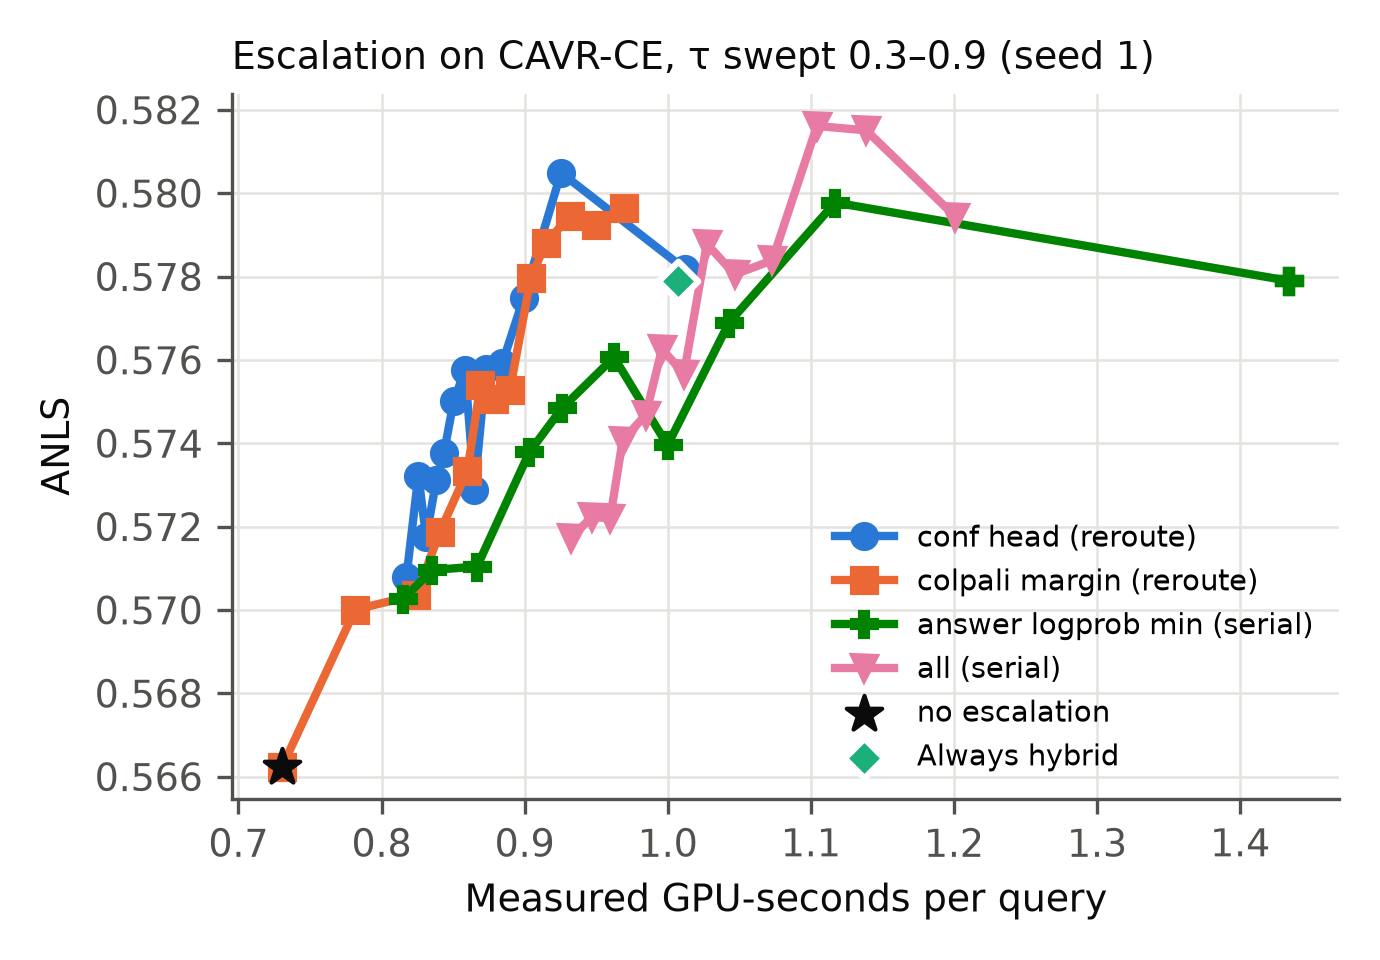
\includegraphics[width=\columnwidth]{figures/escalation.png}
  \caption{Escalation on CAVR-CE: answer quality against measured GPU cost as $\tau$ is swept (seed 1).}
  \label{fig:escalation}
\end{figure}

\subsection{Scalability, throughput and energy}
\label{sec:res-scale}

\paragraph{Serving under load.} A Poisson load test with dynamic batching, simulated from the measured per-query
service times and measured batching curves, gives the highest arrival rate one GPU sustains at p95 $\le$ 2\,s and
the number of GPUs needed for a given load (Table~\ref{tab:load_test}, mean over seeds; Figure~\ref{fig:gpus},
seed 1). Serving 100 queries/s at p95 $\le$ 2\,s needs 106.0 $\pm$ 0.6 GPUs for always-hybrid,
72.4 $\pm$ 3.9 for CAVR-CE (32\% fewer), 64.4 $\pm$ 0.5 for always-visual and
41.6 $\pm$ 0.8 for the oracle. With HF Transformers generation, one GPU serves at most 3.88 (text),
3.06 (visual) and 1.80 (hybrid) queries/s at the best batch size within memory.

\paragraph{Visual index scaling.} ColPali stores 1,031 vectors per page. At 100k pages the index needs
24.6\,GiB in bf16, more than the 24\,GiB of one GPU before any model weights or activations
(Table~\ref{tab:index_scaling}, Figure~\ref{fig:index}). Streaming it from pinned host memory costs
1044\,ms per query; 2$\times$2 pooling shrinks it to 6.3\,GiB and 10.3\,ms
but lowers recall@1 on the real corpus from 0.577 to 0.525 (both measured with the same batched
query encoding); sharding over 2 GPUs gives 19.8\,ms (emulated by timing the shards one
after another on one GPU). A GPU-resident index answers in 0.55\,ms at 1k pages and 19.8\,ms at
50k pages. Building a 100k-page index would take about 1.7 GPU-hours, extrapolated from a 64-page
benchmark at batch 4 (16.2 pages/s); the 1,786-page evaluation index was built at batch
8, which exceeded GPU memory, and ran at 11.3 pages per GPU-second. docTR OCR of the
1,786 evaluation pages took 471\,s and 29.3\,kJ.

\paragraph{Router overhead.} The CAVR router (mpnet embedding and MLP) takes 11.7\,ms per query at
batch 1 on the GPU (25.0\,ms on the CPU) and reaches 12,454 queries/s at large
batch. CAVR-CE takes 24.8\,ms and 1.74\,J per query at batch 1, and its cross-encoder sustains
389 queries/s. Neither is a bottleneck next to generation (Table~\ref{tab:router_throughput}).

\begin{table}[t]
\centering
\caption{Serving capacity from a Poisson load test with dynamic batching (simulated from measured service times on one RTX 4090): highest arrival rate one GPU sustains at the p95 target, and GPUs needed to hold p95 $\leq$ 2\,s at a given load.}
\label{tab:load_test}
\begin{tabular}{lrrrrrr}
\toprule
\textbf{Policy} & \textbf{QPS@p95$\leq$2s} & \textbf{QPS@p95$\leq$5s} & \textbf{GPUs@10} & \textbf{GPUs@25} & \textbf{GPUs@50} & \textbf{GPUs@100} \\
\midrule
Always text & 2 & 3 & 4 & 10 & 21 & 39 \\
Always visual & 0.75 & 1.75 & 8 & 18 & 34 & 65 \\
Always hybrid & 0.25 & 1 & 14 & 30 & 55 & 106 \\
Keyword rule (submitted) & 1.75 & 2.75 & 5 & 10 & 20 & 40 \\
CAVR & 0.75 & 1.5 & 8 & 19 & 35 & 67 \\
Per-query oracle & 1.25 & 2.5 & 5 & 11 & 22 & 42 \\
CAVR-CE, val-chosen lambda & 0.5 & 1.25 & 9 & 21 & 39 & 74 \\
\bottomrule
\end{tabular}
\end{table}

\begin{table}[t]
\centering
\caption{CAVR operating points ($\lambda$ is set at run time): test ANLS, capacity of one GPU and GPUs needed at p95 $\leq$ 2\,s (seed 1).}
\label{tab:load_test_ops}
\begin{tabular}{lrrrrrr}
\toprule
\textbf{Policy} & \textbf{ANLS} & \textbf{QPS/GPU} & \textbf{GPUs@10} & \textbf{GPUs@25} & \textbf{GPUs@50} & \textbf{GPUs@100} \\
\midrule
CAVR, $\lambda$=0.0 & 0.577 & 0.25 & 13 & 28 & 52 & 101 \\
CAVR, $\lambda$=0.02 & 0.571 & 0.25 & 12 & 26 & 49 & 93 \\
CAVR, $\lambda$=0.05 & 0.555 & 0.25 & 10 & 22 & 41 & 79 \\
CAVR, $\lambda$=0.1 & 0.550 & 0.75 & 8 & 19 & 35 & 67 \\
CAVR, $\lambda$=0.2 & 0.551 & 0.75 & 8 & 18 & 32 & 64 \\
CAVR + ret. scores, $\lambda$=0.0 & 0.578 & 0 & 14 & 30 & 55 & 106 \\
CAVR + ret. scores, $\lambda$=0.02 & 0.578 & 0.25 & 13 & 29 & 53 & 102 \\
CAVR + ret. scores, $\lambda$=0.05 & 0.574 & 0.25 & 11 & 24 & 46 & 86 \\
CAVR + ret. scores, $\lambda$=0.1 & 0.550 & 0.5 & 8 & 18 & 35 & 67 \\
CAVR + ret. scores, $\lambda$=0.2 & 0.545 & 0.75 & 8 & 17 & 31 & 61 \\
CAVR-CE, $\lambda$=0.0 & 0.576 & 0.25 & 11 & 26 & 47 & 91 \\
CAVR-CE, $\lambda$=0.02 & 0.574 & 0.25 & 10 & 23 & 43 & 83 \\
CAVR-CE, $\lambda$=0.05 & 0.569 & 0.25 & 9 & 21 & 40 & 78 \\
CAVR-CE, $\lambda$=0.1 & 0.565 & 0.5 & 9 & 19 & 38 & 71 \\
CAVR-CE, $\lambda$=0.2 & 0.554 & 0.75 & 8 & 18 & 34 & 66 \\
\bottomrule
\end{tabular}
\end{table}

\begin{table}[t]
\centering
\caption{ColPali index scaling on one RTX 4090: p50 query latency (ms, batch 1). Pooling 2$\times$2 cuts vectors per page 1031$\to$263; R@1 on the real corpus 0.577$\to$0.525. Sharded latency is emulated (shards timed one by one on one GPU).}
\label{tab:index_scaling}
\begin{tabular}{lrrrrrr}
\toprule
\textbf{Pages} & \textbf{Index GiB} & \textbf{GPU} & \textbf{CPU stream} & \textbf{Pooled GiB} & \textbf{Pooled GPU} & \textbf{GPUs / sharded} \\
\midrule
1,000 & 0.2 & 0.5 & -- & 0.1 & 0.3 & 1 / -- \\
10,000 & 2.5 & 4.1 & 104.5 & 0.6 & 2.4 & 1 / -- \\
50,000 & 12.3 & 19.8 & 522.4 & 3.1 & 5.3 & 1 / -- \\
100,000 & 24.6 & -- & 1044.1 & 6.3 & 10.3 & 2 / 19.8 \\
\bottomrule
\end{tabular}
\end{table}

\begin{table}[t]
\centering
\caption{Router (mpnet embedding + CAVR MLP) on one RTX 4090: batch-1 p50 11.7\,ms; throughput by batch size. CAVR-CE (embedding + passage selection + cross-encoder): batch-1 p50 24.8\,ms, 1.74\,J per query; cross-encoder throughput up to 389 queries/s.}
\label{tab:router_throughput}
\begin{tabular}{lrr}
\toprule
\textbf{Batch} & \textbf{Latency (ms)} & \textbf{Queries/s} \\
\midrule
1 & 11.66 & 86 \\
2 & 13.30 & 150 \\
4 & 13.20 & 303 \\
8 & 13.33 & 600 \\
16 & 13.91 & 1,151 \\
32 & 14.63 & 2,187 \\
64 & 15.32 & 4,178 \\
128 & 17.06 & 7,503 \\
256 & 21.98 & 11,646 \\
512 & 41.11 & 12,454 \\
1024 & 85.06 & 12,039 \\
\bottomrule
\end{tabular}
\end{table}

\begin{figure}[t]
  \centering
  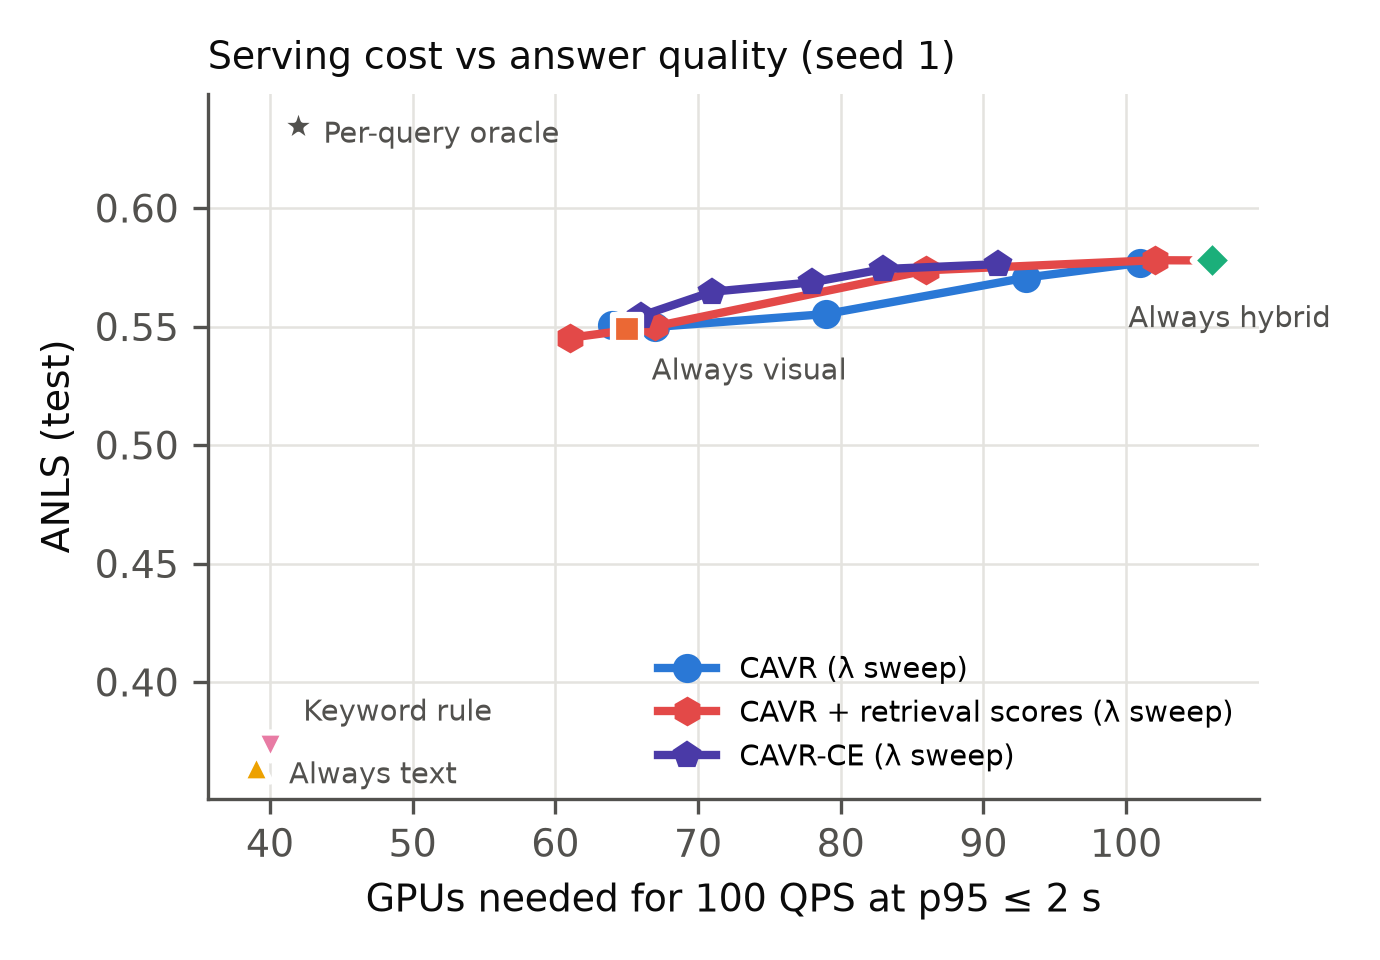
\includegraphics[width=\columnwidth]{figures/gpus_vs_quality.png}
  \caption{GPUs needed to serve 100 queries/s at p95 $\le$ 2\,s against answer quality (seed 1).}
  \label{fig:gpus}
\end{figure}
\begin{figure}[t]
  \centering
  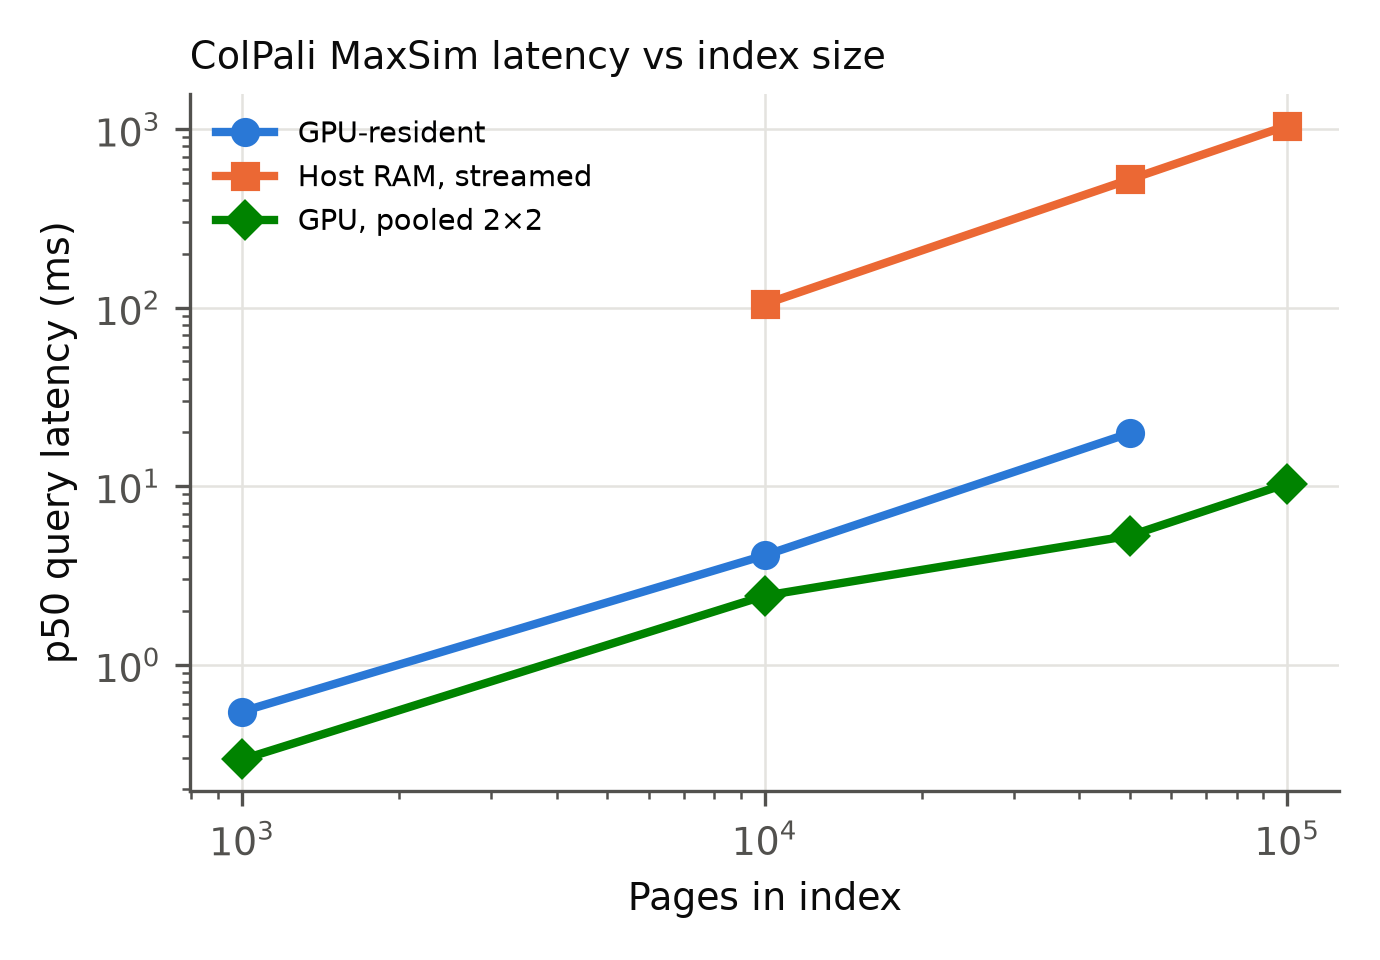
\includegraphics[width=\columnwidth]{figures/index_scaling.png}
  \caption{ColPali MaxSim query latency against index size for a GPU-resident, host-streamed and pooled index.}
  \label{fig:index}
\end{figure}

\subsection{Limitations}
\label{sec:res-limits}

All measurements use one consumer GPU (GeForce RTX 4090) under Windows; caps on visual tokens and OCR length keep memory
below the point where the driver spills to system RAM. Generation uses HF Transformers rather than a serving
engine such as vLLM, so absolute capacity is pessimistic; the comparison between policies is the main result.
The load test is a simulation driven by measured service times, not live traffic, and escalation latencies are
computed from measured per-stage times rather than measured on concurrent workers. Indexes of 10k--100k pages
repeat the real page embeddings, which is valid for latency and memory but not for retrieval quality at that
scale, and multi-GPU sharding is emulated on one GPU. Energy covers the GPU only (NVML). The router handles text
queries over visual documents; queries that contain an image are out of scope. Finally, the 35\% of
queries that every path fails bound what routing can achieve on this benchmark.
